\documentclass[00_mcda_tutorial.tex]{subfiles}

\begin{document}
\section*{Tutorial 3: multi-criteria decision analysis}
\addtocounter{section}{1}
\addcontentsline{toc}{section}{\protect\numberline{}Tutorial 3: multi-criteria decision analysis}

\subsection*{Subjects covered}
\begin{itemize}
  \item Creating a new workspace based on an example dataset
  \item Exploring different methods for preference elicitation, that is, quantifying how important the benefits and risks of treatments are to you
  \item Seeing how these preferences impact the relative value of the evaluated treatments
\end{itemize}


\subsection*{Sign in to your organisation's ADDIS/MCDA.}
\leftpointright \, Open your browser and navigate to \href{https://mcda.drugis.org}{https://mcda.drugis.org}.
Use your Google account to sign in.

\begin{sidebar*}
In case of the enterprise edition, navigate to the URL provided by your organisation. Use your username and password to sign in.
\end{sidebar*}

You will be redirected to your personal homepage, containing your previously created workspaces, both finished and unfinished (if any).

\subsection*{Create the example workspace}
\leftpointright \, Click the ‘Create workspace’ button. In the dialog that appears, choose ‘Select tutorial workspace’. Now select the ‘Zinbryta initial assessment simplified’ option in the dropdown and press ‘add’. You should now be on the Overview screen of a fresh workspace, like on Figure \ref{fig:overview_page}.
\newline

\begin{figure}[!h]
  \centering
  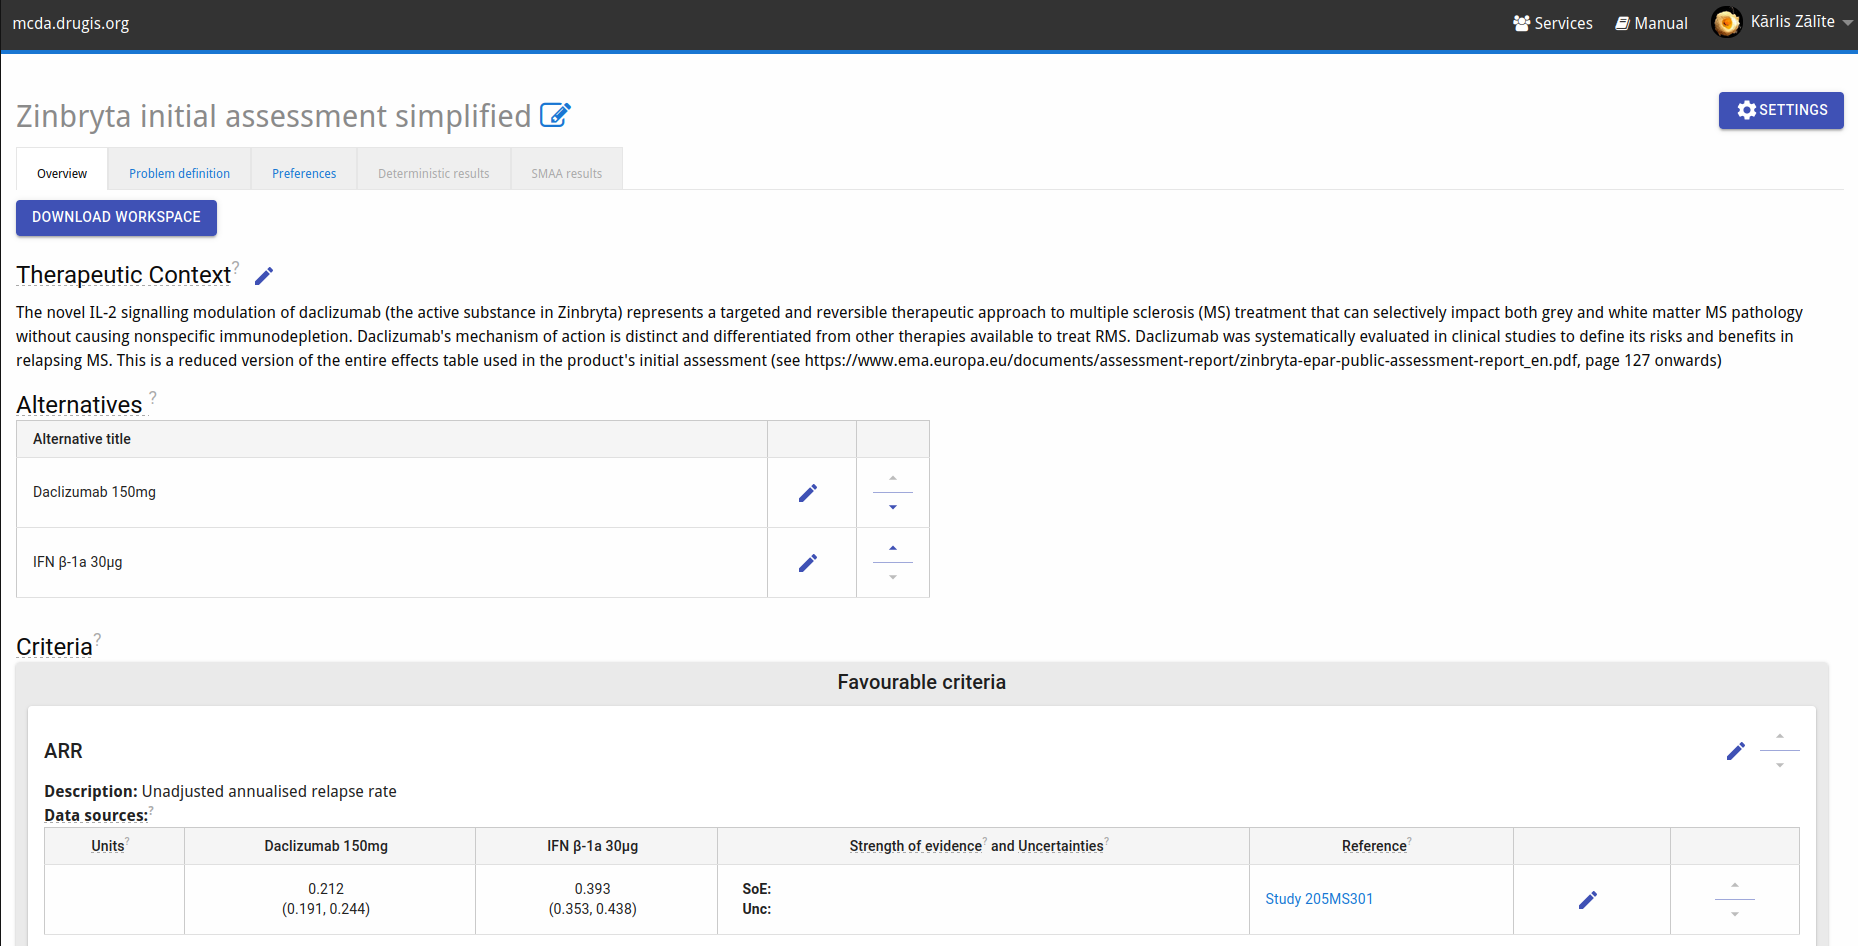
\includegraphics[width=\textwidth]{fig/overviewPage.png}
  \caption{The overview page}
  \label{fig:overview_page}
\end{figure}

\noindent \faGraduationCap \, The overview screen shows you the criteria and their data sources, the alternatives, and the table with measurement data.
\newline

\noindent \faLightbulbO \, Many elements in the interface have a contextual help icon (Figure \ref{fig:tooltip}) that you can click for explanation and links to the relevant section in the manual.
\newline

\begin{figure}[!h]
  \centering
  
\includegraphics[width=.3\textwidth]{fig/contextHelp.png}
  \caption{Contextual help icon, outlined in red}
  \label{fig:tooltip}
\end{figure}

\noindent \faGraduationCap \, The example concerns a simplified version of the \href{https://www.ema.europa.eu/en/medicines/human/EPAR/zinbryta#authorisation-details-section}{Zinbryta assessment}. The criteria are the primary endpoint (Annualised Relapse Rate) and several adverse events. Only data from the 205MS301 study are included, as can be seen in the effects table. The references column contains links to the clinicaltrials.gov registry version of this study in case you want to look at the source data.

\subsection*{Evaluate evidence}
\leftpointright \, Go to the ‘Problem definition’ tab and take a moment to look at the effects table. Do you have a clear preference for one of the two treatments? What makes this treatment better in your view?
\newline

\noindent We are now going to quantify your preferences in several ways to see whether your intuitive answer in the previous step matches the outcome of the MCDA.
\newline

\noindent \faGraduationCap \, MCDA is a quantitative approach to benefit-risk assessment and ranks the evaluated treatments from least to most preferable. How preferable a treatment is, is reflected by its utility score. In ADDIS, a treatment’s utility score is the sum of its per-criterion utility values. This method is called the additive value model.
\newline

\noindent \faGraduationCap \, Utility, as a constructed measure of well-being, has no natural scale. For simplicity, ADDIS (arbitrarily) uses the scale from 0 to 1, with 0 meaning the worst and 1 the best possible combination of the criteria scale values.

\subsection*{Preferences: partial value functions}
\leftpointright Go to the ‘Preferences’ tab.
\newline

\noindent \faGraduationCap \, At the top are the partial value functions, which indicate how utility changes as a function of the criteria scale values. Below this is the weights section which is the main focus of this tutorial. Before setting weights, the partial value functions need to be defined.
\newline

\noindent \leftpointright \, Click on the ‘Decreasing’ button for ARR. Lower relapse rate is better, and we are going to assume that utility changes linearly with the relapse rate.

\noindent The range over which the partial value functions are defined depends on the data included in the effects table. These ranges can be modified in the ‘Problem definition’ tab, but this goes beyond the scope of this tutorial.
\newline

\noindent \leftpointright \, Also define linear partial value functions for the adverse event criteria, with low values being best. The result should look like Figure \ref{fig:preferences}.
\newline

\begin{figure}[!h]
  \centering
  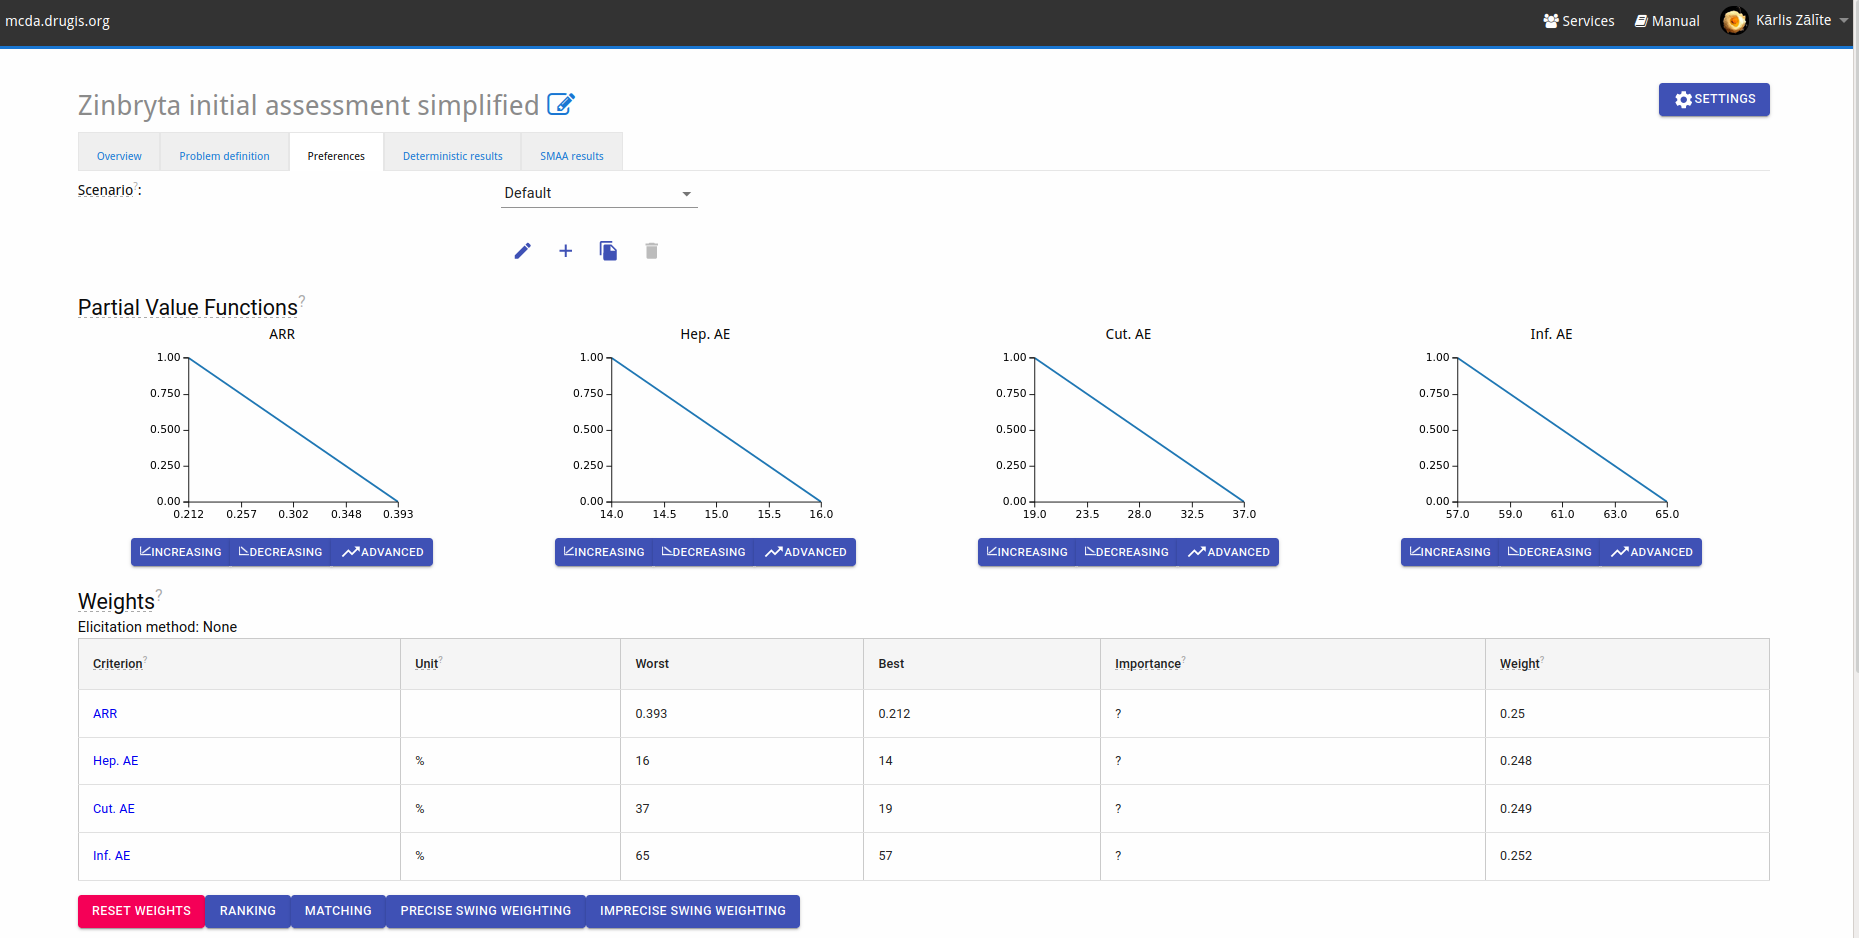
\includegraphics[width=\textwidth]{fig/preferences.png}
  \caption{The preferences tab after setting the partial value functions}
  \label{fig:preferences}
\end{figure}

\noindent \leftpointright \, (optional) Explore the process for defining non-linear partial value functions by clicking the ‘Advanced’ button under any of the functions, and adjusting the sliders. You can leave the definition process at any time by clicking on the ‘Cancel’ button.
\newline

\noindent \faGraduationCap \, Non-linear partial value functions are needed when equivalent changes on a criterion’s measurement scale do not result in equivalent changes in utility.  For example, one can imagine that going from severe depression to mild depression is more valuable than improving from mild to no depression (diminishing marginal utility).

\subsection*{Preferences: ranking elicitation}
First let’s see how the treatments compare if we only give an ordinal ranking, with efficacy as the most important.
\newline

\noindent \leftpointright \, Click the ‘Ranking’ button below the weights table, then indicate that ARR is the most important criterion, followed by Hep. AE, then Inf. AE. Then click on the ‘Deterministic results’ tab.
\newline

\noindent \faGraduationCap \, The deterministic results screen shows the effects table, with values that can be changed to perform sensitivity analysis (subject of a later tutorial). Below this are the representative weights, showing which weights the system has used to calculate the value profiles. Because we did not supply direct numerical weights but did ordinal ranking instead, the system has generated a default set of weights consistent with the ranking provided. These so-called representative weights are shown in the table.
\newline

\noindent \faGraduationCap \, The total value indicates an alternative’s overall utility according to the weights you supplied and the data in the effects table. The value profile plot below the total value table shows the contributions of each criterion to these overall utility values (Figure \ref{fig:deterministic_ranked}). In the current situation, we can see that Daclizumab is much better at reducing the relapse rate, while the other treatment is better as far as all the adverse events goes. Because we have indicated that ARR is much more important than the adverse events, it follows that we should prefer Daclizumab.

\begin{figure}[!h]
  \centering
  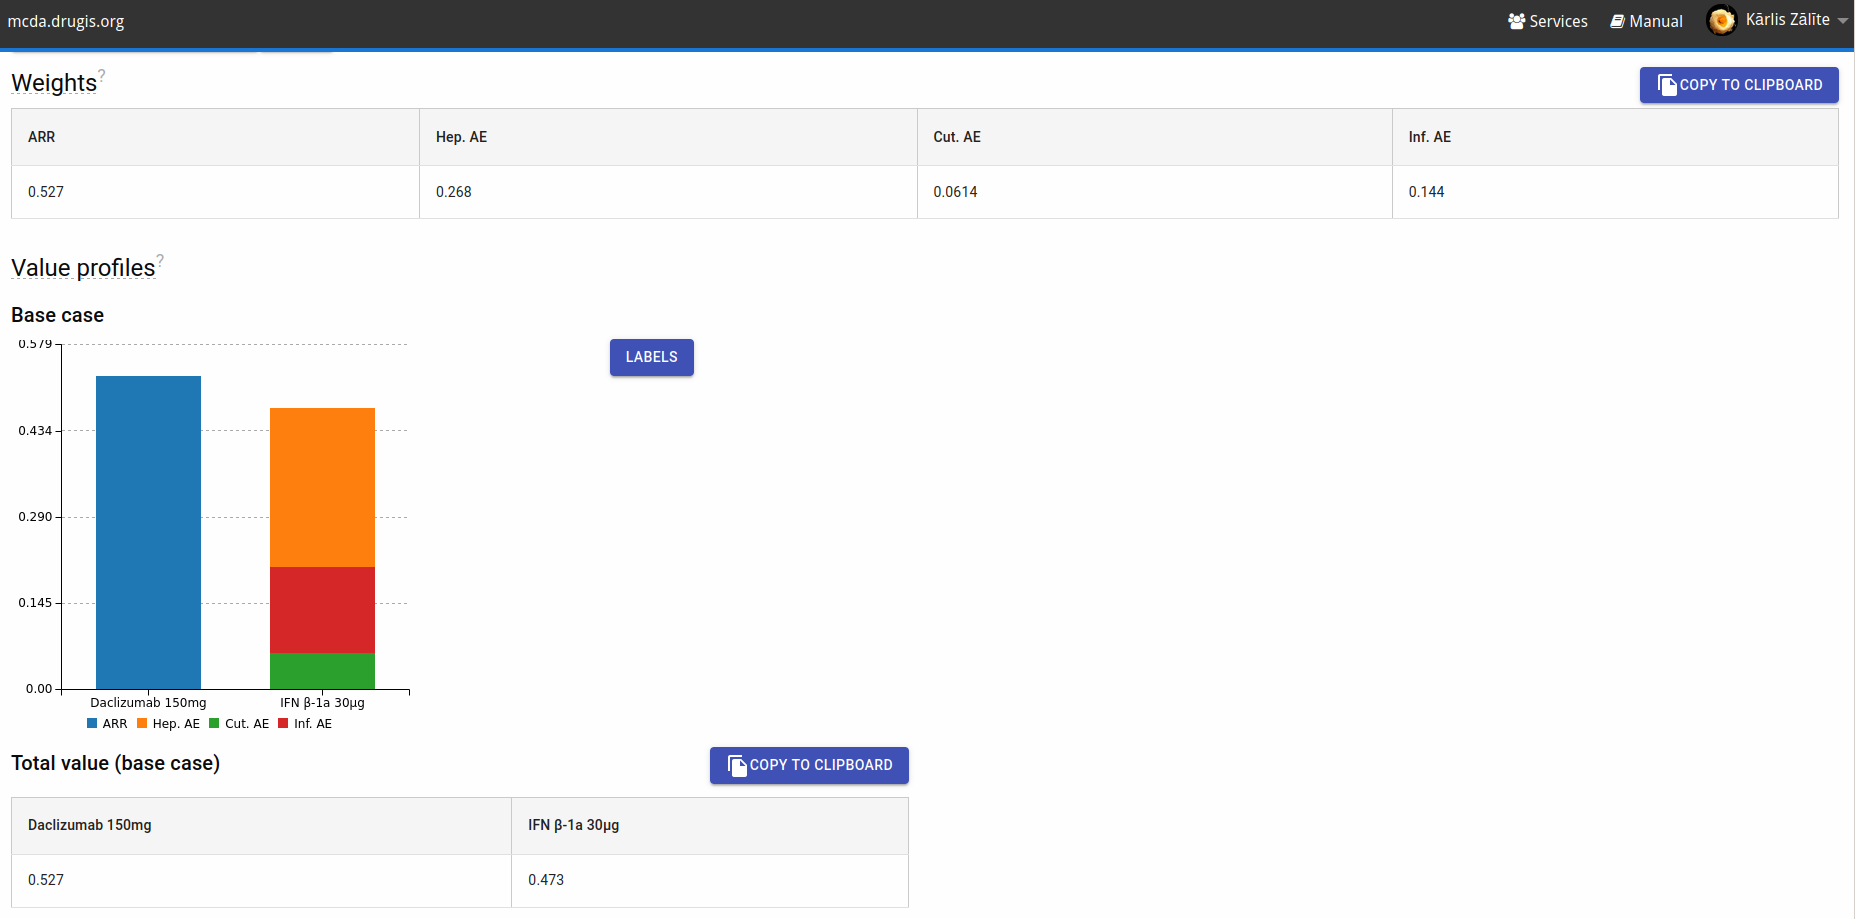
\includegraphics[width=\textwidth]{fig/deterministicRanked.png}
  \caption{Deterministic analysis}
  \label{fig:deterministic_ranked}
\end{figure}

\subsection*{Preferences: equal weights}
Let’s see how the picture changes if we weight all criteria equally.
\newline

\noindent \leftpointright \, Go back to the ‘Preferences’ tab, and click the copy icon next to the scenario dropdown (Figure \ref{fig:copy_scenario}). Give the new scenario an intuitive name like ‘Equal weights.’
\newline

\begin{figure}[!h]
  \centering
  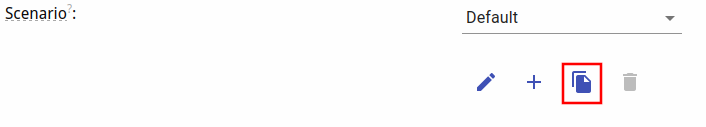
\includegraphics[width=.5\textwidth]{fig/copyScenario.png}
  \caption{Copy scenario button}
  \label{fig:copy_scenario}
\end{figure}

\noindent \faGraduationCap \, Scenarios let you save different configurations of partial value functions and weights, and allow you to switch between them at will. New scenarios can be created as either a copy of the currently selected one, or completely blank, i.e. without defined partial value functions  and weights.
\newline

\noindent \leftpointright \, Click the ‘Precise Swing weighting’ button below the weights table, indicate that ARR is the most important, and then leave all the sliders at 100\% and click ‘Save’. Now navigate to the ‘Deterministic results’ tab again, and the results should be quite different. The representative weights are 0.25 for each criterion, and IFN $\beta$-1a 30$\mu$g is now better than Daclizumab. Because there are simply more adverse event criteria, they together outweigh the higher effectiveness of Daclizumab.
\newline

\noindent \faLightbulbO \, You can switch between scenarios using the dropdown at the top of the tab, and the results will reload.
\newline

\noindent \faGraduationCap \, Precise Swing weighting lets you manually and precisely set the weights of all criteria relative to the most important one, as you have just done. Leaving all weights at 100\% means they are all equally important. Imprecise Swing weighting similarly lets you set the weights, but allows you to specify probable intervals for the weights, for when you are less certain about your preferences or wish to see the consequences in stochastic analysis of uncertain weights.

\subsection*{Preferences: matching elicitation}
You can also determine your preferences by comparing alternative outcome scenarios, in the Matching elicitation process.
\newline

\noindent \leftpointright \, Click the ‘Matching’ button under the weights table on the preferences tab. Select ‘ARR’ as the most important criterion in Step 1. In the following steps, you are presented with two alternative scenarios, A and B (Figure~\ref{fig:matching1}). Change the value for ARR in Alternative B by moving the slider until you feel that the two alternatives are approximately equal, e.g. decreasing ARR by a certain amount is ‘worth’ about that much increase in Hep. AE. Then click ‘Next’ until you have completed the elicitation. The Weights table will now have updated with the corresponding importances and weights.
\newline

\begin{figure}[!h]
  \centering
  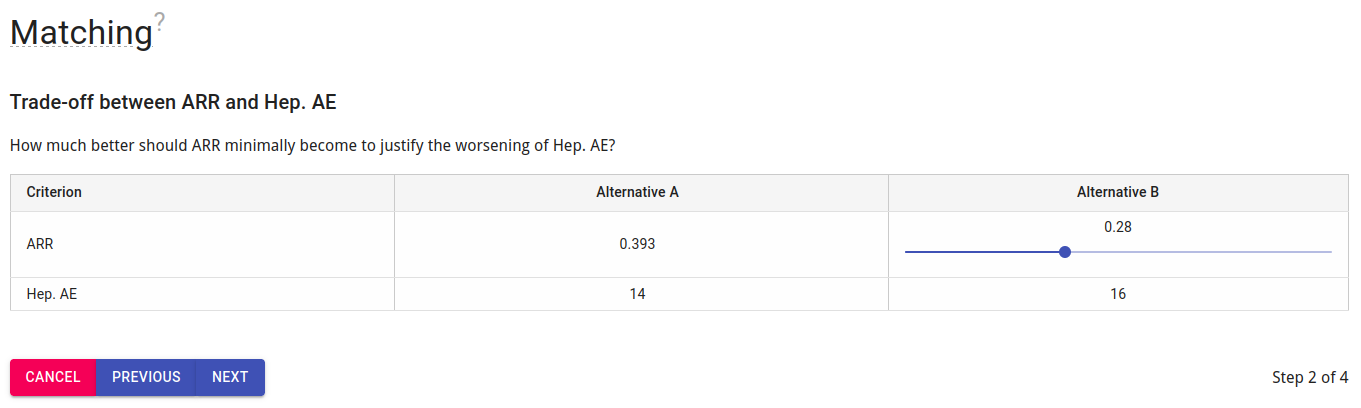
\includegraphics[width=\textwidth]{fig/matching1.png}
  \caption{Matching elicitation (for one tradeoff)}
  \label{fig:matching1}
\end{figure}

\noindent \leftpointright \, Go to the Deterministic results tab to see how the values of the treatments have changed. Are these results in line with your intuitive assessment at the beginning of the tutorial?

\noindent \leftpointright \, After finishing filling out your preferences in the Matching elicitation, go to the Deterministic results tab to see how the values of the treatments have changed. Are these results in line with your intuitive assessment at the beginning of the tutorial?


\begin{sidebar*}

\subsection*{Further elicitation methods (Enterprise edition)}

We will here briefly cover additional elicitation methods which are only available in the enterprise edition.
\newline

\noindent \leftpointright \, Go to the Preferences tab, and create a new scenario called 'Threshold' that is a copy of the 'Equal weights' scenario you created earlier. This lets you avoid having to set the PVFs again. Click the 'Threshold' button.
\newline


\noindent \faGraduationCap \, The Threshold technique for preference elicitation is similar to matching elicitation, with users being asked to weigh alternatives against each other based on quantitative changes in each criterion. The difference is that the user is first asked what magnitude of change in the primary criterion they find most logical to reason about.
\newline

\noindent \leftpointright \, In step 1, choose `ARR` as your reference criterion. Use an improvement by 0.05 as your reference change.
\newline

\noindent \leftpointright \, In step 2 (Figure~\ref{fig:threshold}), adjust the changes for each other criterion so that, in your opinion, that criterion's change is approximately equivalent to an improvement of 0.05 in ARR.
\newline

{
	\centering
    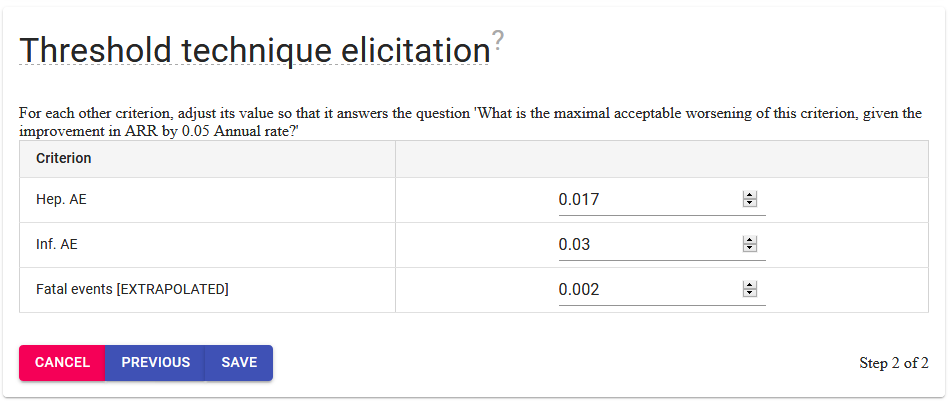
\includegraphics[width=\textwidth]{fig/threshold.png}
    \captionof{figure}{Threshold technique elicitation, step two: setting equivalent changes.}
    \label{fig:threshold}
    \par
}

\noindent \leftpointright \, Click 'Save' and inspect the new weights. Do they differ greatly from those you got for previous elicitation methods? Go to the 'Deterministic' tab and contrast the values of the different alternatives. Switch to one of your other scenarios and contrast the outcomes with those of your threshold weights.
\newline

\noindent \leftpointright \, Go to the Preferences tab, and create a new copy of the 'Equal weights' scenario, called 'Choice-based matching'. Click the 'Choice-based matching' button.
\newline

\noindent \faGraduationCap \, The choice-based matching elicitation method uses an automatically-generated series of questions to approximate the user's preferences. Each question presents two alternative scenarios, and the user is asked which one they prefer. The questions are generated in such a manner that the system's uncertainty about the preferences is minimised as they are answered. This process is somewhat more labourious than adjusting a single value for each criterion, as in several other elicitation techniques. However, some users prefer being asked to judge alternatives over having to provide a numerical value directly.
\newline

\noindent \leftpointright \, Answer the questions (Figure~\ref{fig:cbmatching}) as they are presented to you. Once you are done, as always contrast the generated weights and their consequences with your previous experiences.
\newline

{	
	\centering
  	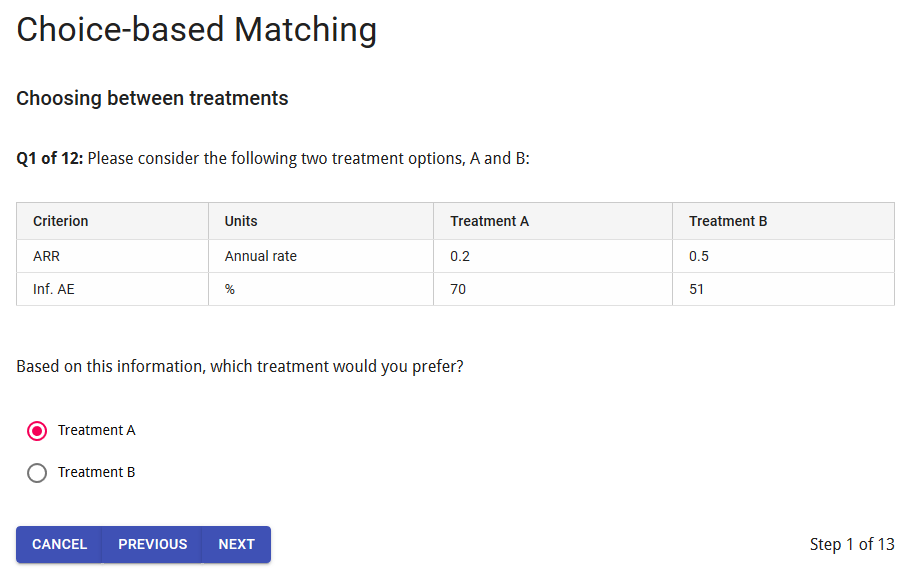
\includegraphics[width=\textwidth]{fig/cbmatching.png}
  	\captionof{figure}{Choice-based matching elicitation example question, asking to judge which alternative is better.}
  	\label{fig:cbmatching}
	\par
}

\end{sidebar*}

\subsection*{Final words}
This tutorial has demonstrated how assigning different importance to criteria can drastically change the relative value of the evaluated treatments. We’ve also shown how quantifying these importances makes it easy to see where these differences originate. Finally, we’ve shown that in the MCDA interface it is easy to input different preference scenarios with different elicitation methods, and switch between them.

\end{document}
